\documentclass[12pt]{article}

% fonts

\usepackage[T1]{fontenc}
\usepackage[full]{textcomp}
\usepackage{newtxtext}
\usepackage{cabin} % sans serif
\usepackage[varqu,varl]{inconsolata} % sans serif typewriter
\usepackage[final,expansion=alltext]{microtype}
\usepackage[english]{babel}
\usepackage{amsmath}
\usepackage[bigdelims,vvarbb]{newtxmath} % bb from STIX
\usepackage[cal=boondoxo]{mathalfa} % mathcal
\usepackage{csquotes}
\usepackage{graphicx}

\usepackage[backend=bibtex,style=numeric]{biblatex}
\bibliography{traffic} % Specify your BibTeX file

% geometry of the page

\usepackage[top=1in,
            bottom=1in,
            left=1in,
            right=1in]{geometry}


% paragraph spacing

\setlength{\parindent}{0pt}
\setlength{\parskip}{2ex plus 0.4ex minus 0.2ex}


\author{Matthew McAnear}
\title{Traffic Fatality Risk by Advanced Safety Features}

% useful packages

\begin{document}

\maketitle

\begin{abstract}
    Despite the proliferation of AI technology in passenger cars of collision detection/avoidance, lane drift systems, and
    various other safety systems, pedestrian and cyclist deaths are NOT significantly reduced by these
    interventions.
\end{abstract}


\section{Introduction}

The National Highway Traffic Safety Administration (NHTSA) reports that, as of preliminary reports through
June of 2023, traffic accidents involving fatalities, in aggregate, are down about 3\%. This decrease is positive,
but looking only at changes from year to year hides the true scale of the problem for vulnerable non-vehicle
road users. While the overall change for pedestrians is also 3\%, the baseline level of risk for pedestrians is
much higher than for passenger vehicles or even for pedalcyclists. Among accidents involving pedestrians, the fatality
range anywhere from a 14\% to 23\% baseline fatality rate throughout the year, depending on the month in
question \cite{national_highway_traffic_safety_administration_early_2024}.

This fatality rate is influenced heavily by the mass of the car\cite{evans_car_1992}. This means that there
are offsetting effects of both increasing vehicle mass and increasing
vehicle saftey. For people outside of the vehicle, however, the statistics are alarming. According to Tyndall,
"between 2010 and 2021 the number of pedestrians killed annually in collisions increased by 72\%, from 4300 to
7400 \cite{tyndall_effect_2024}." Due to relaxed emissions standards for small trucks compared to passenger cars,
American buyer preferences shifted toward sport utility vehicles (SUVs) and trucks \cite{kovach_rise_2021}. Taken into
account this connection between both the proliferation of large vehicles and the clear connection in fatality risk to
more massive and taller vehicles\cite{tyndall_effect_2024}, finding the factors that minimize pedestrian fatalities
is of critical importance for public health.

It is common knowledge that AI systems have become an increasing part of every day life, and passenger
vehicles are no exception. The question is if these improved safety systems are reducing the risk of fatalities
among pedestrians and cyclists. Next, assuming these new systems yield tangible improvements to pedestrian safety,
are the improvements large enough in magnitude to offset the increased risk from the size and height of vehicles?

In this paper, we focus primarily on those factors that influence the risk of fatalities in crashes involving pedestrians
and cyclists. After controlling for the effect of weather conditions,
geographic region, and crash variables such as time of day and intersection type, we estimate the effect
of advanged safety features on the risk of pedestrian and cyclist fatalities within vehicle types.


\section{Data}

Our data comes from the US National Highway Traffic Safety Administration (NHTSA). The NHTSA collects and distributes
crash statistics on fatal accidents through FARS, the Fatal Accident Reporting System, and CRSS, the Crash Report
Sampling System. Through these two datasets, we can investigate risk factors for fatal accidents and injuries in
pedestrian and cyclist accidents. All files are available at
    [the NHTSA website](https://www.nhtsa.gov/file-downloads?p=nhtsa/downloads/). Several simplifying assumptions must be
made in order to combine the two datasets - for example, the CRSS data is taken from 60 sampling locations, not
nationwide, and weights are applied in order to estimate national level
statistics\cite{national_highway_traffic_safety_administration_crash_nodate}.  To simplify the analysis, we exclude
from consideration crashes involving multiple vehicles and focus solely on single-vehicle collisions with pedestrians
and cyclists. We also further ignore the crash group, i.e. whether the driver or cyclist was at fault, what
specific maneuver was being performed, or where the pedestrian happened to be in relation to the vehicle. These are
important characteristics to consider, but the overall sparsity of the data makes inference in small subgroups
challenging.

% The result of this subsampling is that certain information is not available at the same level of default as the 
% fatality statistics. Namely, states in the fatal crash statistics have to be manually categorized into the 
% same regions reported the CRSS. Beyond this, the names of the columns are slightly different, but the overall 
% structure of the data is otherwise analogous. The dataset is fairly complex, spanning multiple files that cover the 
% accidents, vehicles involved, specific information about the vehicles, and a host of other components. To simplify
% the analysis, we exclude from consideration crashes involving multiple vehicles and focus solely on single-vehicle 
% collisions with pedestrians and cyclists. 

Another potential issue with the dataset is the overall level of sparsity in our features. While there is no
missingness for important crash level statistics such as the bodyclass of the vehicle, things like the weight class
are missing and cannot be reliably imputed. Safety features are also missing for a large number of vehicles; to solve
this, we assume that any safety feature not listed as "standard" is not present. Though we could simulate this data
conditional on other factors, this is an extension to a future analysis and out of scope for this short paper.

We make some other simplifying and data cleaning steps, namely collapsing the bodyclass vehicles into broader categories,
listed in the appendix.

\section{Methodology}

Our model will be a relatively traditional logistic regression, as we are primarily interested in inference on the
effects of our variables of interest and so need a model that retains interpretability. However, we will
add hierarchical structure to account both the full and group-level effects of each covariate across
cyclists and pedstrians. See Figure \ref{fig:model_graph} for a graphical representation of the model.

We wish to estimate the effects of the variables separately for both pedestrians and cyclists, but because of our
relatively sparse feature space, there is some concern of wild coefficient values, so for that reason we use the
hierarchical model to constrain an overall effect of a feature, and then estimate whether that effect differs
between cyclists and pedestrians. The overall effects considered are vehicle bodyclass, lighting conditions, weather
conditions, and vehicle safety features. Each beta coefficient is assumed to follow a Laplace prior. This specification
is equivalent to a LASSO penalty\cite{tibshirani_regression_1996}, and will help to mitigate potential model fitting
estimates due to the sparsity of the feature space.

\section{Results}

We see strong relationships across region and vulnerable road user type (cyclist or pedestrian). According to our
model, there is a roughly

Many of the results are exactly as one would expect, and partially align with our hypothesis. For example, the
coefficient on pickup trucks is strong positive for both cyclists and for pedestrians, indicating that these vehicles
are much more likely to kill a pedestrian or cyclist compared to cars (the baseline group). See
Figure \ref{fig:coefficients}. Many results border on the obvious - the log-odds of a fatality increase the most when
a truck/semi are involved. The trend genereally holds that increase vehicle weight corresponds to an increasing
likelihood of fatality for pedestrians and cyclists. Somewhat surprising is how these effects are manifested across
vulnerable road users. For example, pickups and semis are much more likely to kill a cyclist than a pedestrian. This is
most likely due to the nature of when and where cycling accidents take place, presumably at higher speeds on shared
infrastructure. Unfortunately, the data is missing an estimated speed in roughly 58\% of pedestrian accidents, and so
use of this as a control variable may unfairly bias our results without a more thoughtful imputation scheme.

Outside of the vehicle centric effects, the largest effects is by far if the accident takes place at night, shown in
figures \ref{fig:coefficients} and \ref{fig:all_users}. This effect is roughly the same for pedestrians and cyclists. 
Inclement weather appears to have a negative effect, such that
worse weather actually reduces the log odds of a fatality. This could be due to drivers being more cautious in
inclement weather, and also because we have collapsed a large variety of weather conditions into a single variable.

However, controlling for these factors, it appears that our safety features have relatively small or unclear effects on
the log-odds of a fatality. The clearest effect is the lane-departure warning system, which appears to reduce the
log-odds of a fatality substantially among cyclists. Equally substantially, however, is the effect of lane-keeping
assistance features, which appears to \textit{increase} the log-odds of a fatality among cyclists.

To make sure of these counterintuitive result, we should remember that the sparsity and high-proportion of missingness
in our data inherently means that certain characteristics may suffer from multicollinearity that improperly
assigns weight to the wrong group. This is a natural fit for a model-averaging approach, the results of which are in 
Table \ref{table:bma_results}. Though the model fit in \texttt{R} with the \texttt{BMA} package is simpler
than our hierarchical model, we can see that many of the features with somewhat ambiguous or counterintuitive 
effects

-- Safety Features


Also somewhat surprisingly, the hierarchical specification
reveals that the impact of body cl


\section{Discussion}

-- Strength of coefficients

-- Implications

\section{Conclusion}

-- Sum up

\section{Support}

\begin{figure}
    \centering
    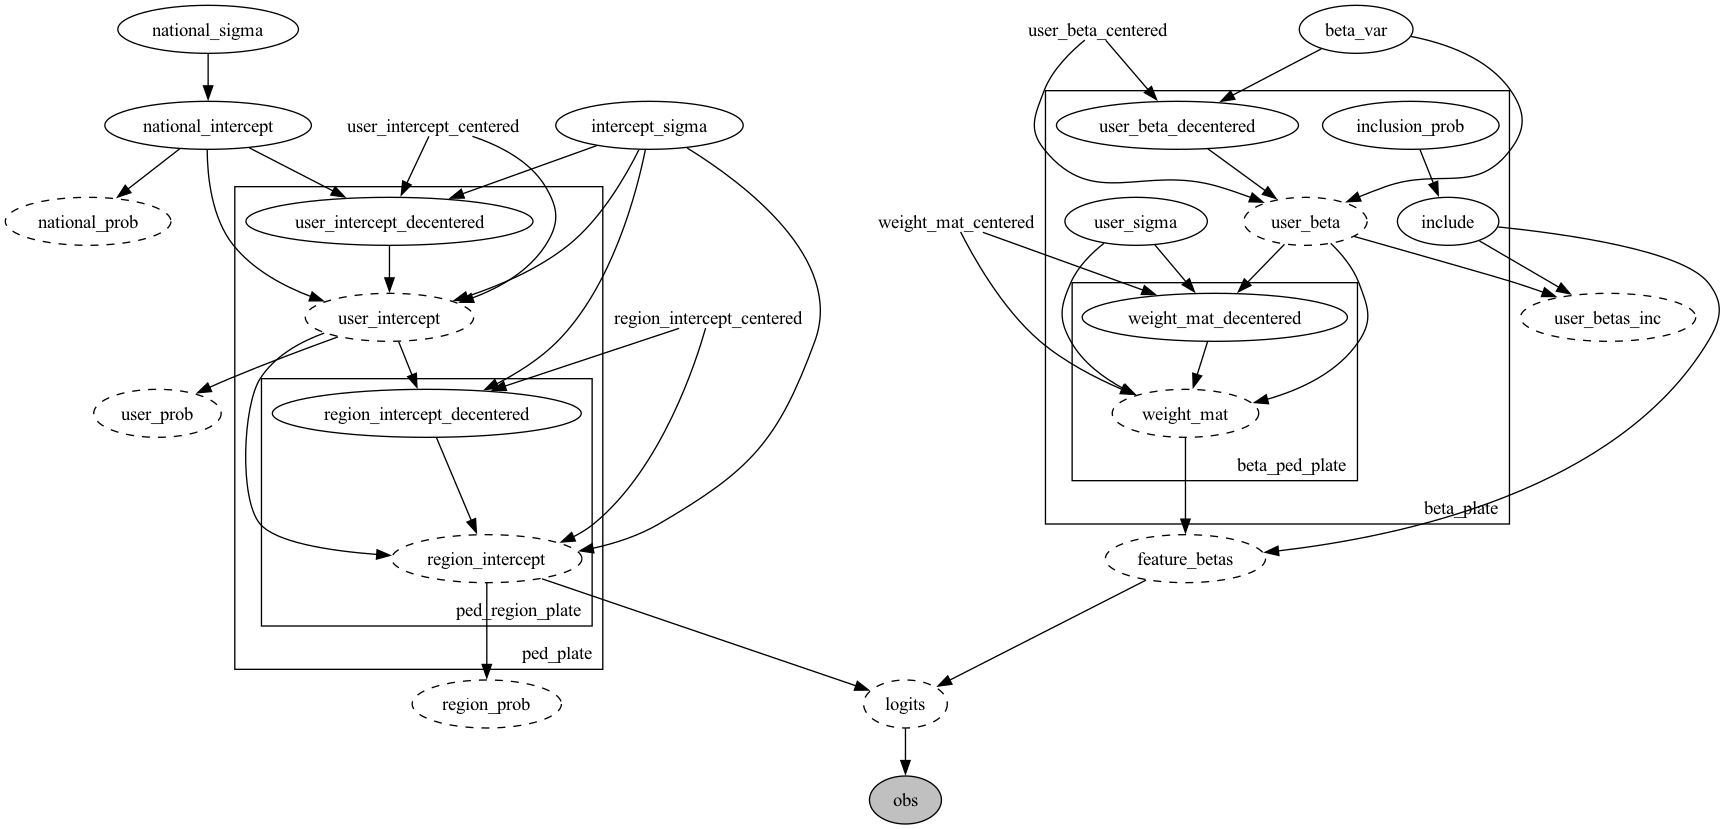
\includegraphics[width=\textwidth]{images/model_graph.png}
    \caption{Graphical representation of the hierarchical logistic regression model.}
    \label{fig:model_graph}
\end{figure}


\begin{figure}
    \centering
    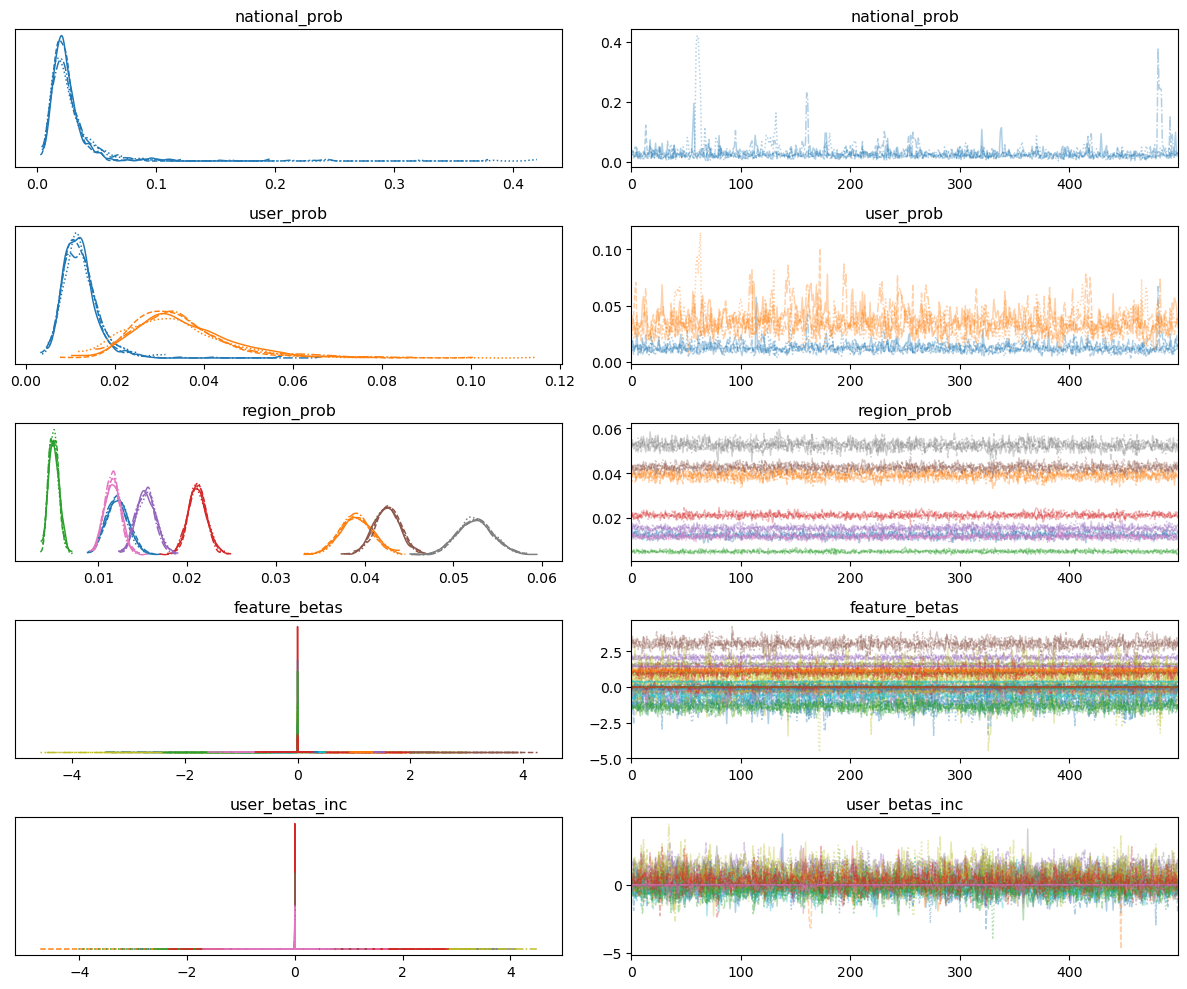
\includegraphics[width=\textwidth]{images/traceplot.png}
    \caption{Traceplot for all variables of interest. Note that there are no divergences and good mixing across all
        chains, indicating that the model has converged across all levels of the hierarchy without major issues.}
    \label{fig:traceplot}
\end{figure}



\begin{figure}
    \centering
    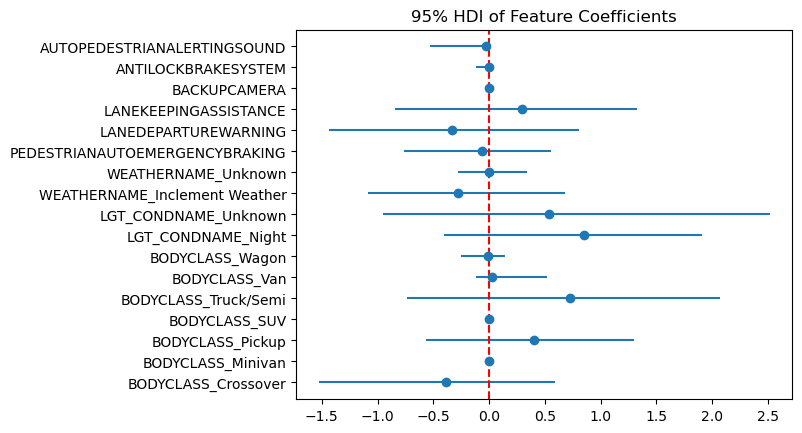
\includegraphics[width=\textwidth]{images/all_users_coefficients.png}
    \caption{Parent-level feature coefficients for variables of interest.}
    \label{fig:all_users}
\end{figure}


\begin{figure}
    \centering
    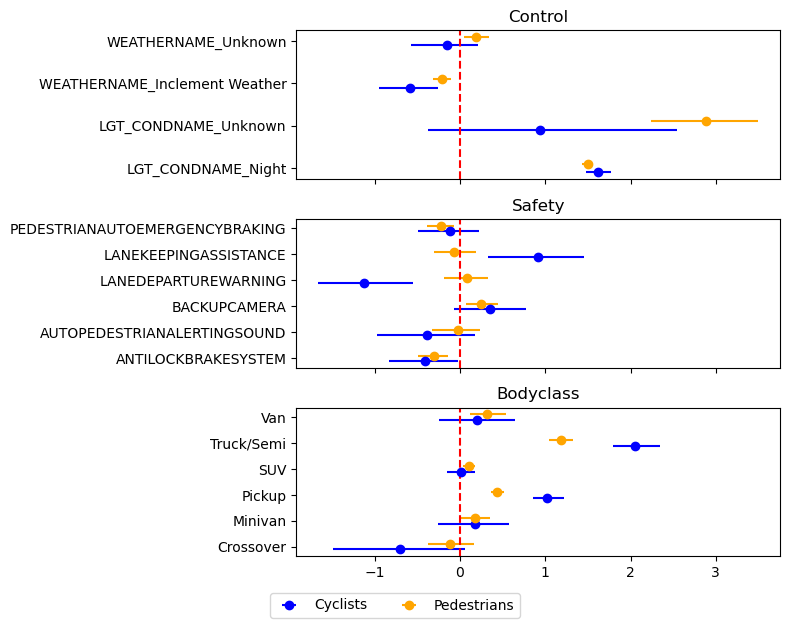
\includegraphics[width=\textwidth]{images/feature_coefficients.png}
    \caption{Feature coefficients for all variables of interest. The coefficients represent the change in the log-odds,
        and error bars represent the 95\% HDI interval.}
    \label{fig:coefficients}
\end{figure}


Prior predictive checks

\printbibliography

\end{document}



%%% Local Variables:
%%% mode: latex
%%% TeX-master: t
%%% End:
